

A Figura~\ref{fig:training} apresenta a distribuição (\textit{boxplot}) e a média com desvio-padrão do \textit{SBERT-score} avaliado no conjunto de teste para os quatro experimentos. Esta métrica calcula a similaridade de cosseno entre os \textit{embeddings} das sentenças, operando teoricamente no intervalo $[-1, 1]$, onde valores próximos a $1$ indicam alta equivalência semântica entre os títulos gerado e de referência.

Os resultados evidenciam uma hierarquia de desempenho coerente com a capacidade de adaptação de cada método. O modelo com treinamento completo (M4) obteve a maior média de \textit{SBERT-score} ($\mu = 0,640$), seguido pelo Q-LoRA (M3) com $\mu = 0,627$. Notavelmente, o ajuste isolado da última camada (M2, $\mu = 0,596$) ficou aquém do \textit{baseline} sem treinamento (M1, $\mu = 0,614$). Esse resultado contraintuitivo pode ser explicado pelo fato de que, ao atualizar apenas a camada de saída mantendo os pesos intermediários congelados, o modelo não desenvolve representações internas adequadas à tarefa, introduzindo um desalinhamento entre as características extraídas pelas camadas ocultas e o comportamento esperado na decodificação.

\begin{figure}[!h]
    \centering
    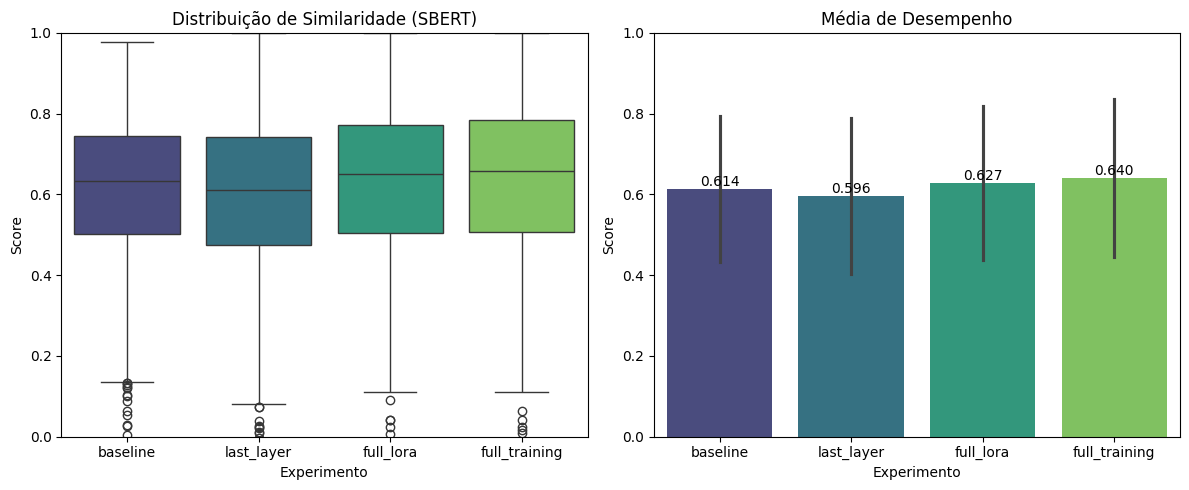
\includegraphics[width=1\linewidth]{figs/training_result.png}
    \caption{Distribuição do \textit{SBERT-score} no conjunto de teste para os quatro métodos avaliados. As caixas representam o intervalo interquartil (IQR) e os losangos indicam as médias amostrais.}
    \label{fig:training}
\end{figure}

Para verificar se as diferenças observadas nas médias são estatisticamente significativas, aplicou-se o teste não-paramétrico de Kruskal-Wallis. A escolha deste teste justifica-se pela violação da premissa de normalidade na distribuição dos \textit{scores} de similaridade, tornando inapropriado o uso de testes paramétricos como a ANOVA. A hipótese nula ($H_0$) postula que as medianas populacionais de todos os grupos são iguais.

O teste global resultou em $H = 30,53$ ($p < 0,001$), rejeitando $H_0$ com alto grau de confiança e confirmando que ao menos um par de métodos apresenta distribuições de desempenho significativamente distintas.

Para identificar quais pares de métodos diferem entre si, aplicou-se o teste \textit{post-hoc} de Mann-Whitney com correção de Bonferroni (nível de significância ajustado $\alpha \approx 0,0083$). Os resultados são apresentados na Tabela~\ref{tab:comparacao_treinamento}.


\begin{table}[H]
\centering
\begin{tabular}{l c c c}
\hline
\textbf{Comparação} & \textbf{Diferença Média} & \textbf{P-valor} & \textbf{Significativo?} \\
\hline
Full Training (M4) vs. Q-LoRA (M3)     & 0,0129 & 0,11    & Não \\
Full Training (M4) vs. Baseline (M1)   & 0,0268 & $<$0,001 & Sim \\
Full Training (M4) vs. Last-Layer (M2) & 0,0447 & $<$0,001 & Sim \\
Q-LoRA (M3) vs. Baseline (M1)          & 0,0138 & 0,08    & Não \\
Q-LoRA (M3) vs. Last-Layer (M2)        & 0,0318 & $<$0,001 & Sim \\
Baseline (M1) vs. Last-Layer (M2)      & 0,0179 & 0,04    & Não$^{*}$ \\
\hline
\end{tabular}
\caption{Resultados do teste \textit{post-hoc} de Mann-Whitney com correção de Bonferroni ($\alpha \approx 0,0083$). $^{*}$Diferença tendencialmente significativa ($p < 0,05$), porém não confirmada após o ajuste para comparações múltiplas.}
\label{tab:comparacao_treinamento}
\end{table}

A análise dos resultados permite extrair três conclusões principais. Primeiramente, a superioridade do treinamento completo sobre métodos fracos foi confirmada, pois o M4 superou estatisticamente tanto o \textit{baseline} quanto o ajuste da última camada ($p < 0,001$ em ambos os casos), ratificando que a atualização irrestrita dos parâmetros é a estratégia mais eficaz para a tarefa estudada. Em segundo lugar, verificou-se a equivalência entre Full Fine-Tuning e Q-LoRA, uma vez que a comparação entre M4 e M3 resultou em $p = 0,109$, indicando ausência de diferença estatisticamente significativa. Este é o achado central do trabalho: o Q-LoRA, que demanda uma fração dos recursos computacionais do treinamento completo, alcança desempenho estatisticamente equivalente ao método mais custoso, validando sua eficiência como alternativa PEFT para cenários com restrições de infraestrutura. Por fim, notou-se a inadequação do ajuste isolado da última camada, visto que a comparação entre M2 e M1 resultou em $p = 0,04$, o qual não é estatisticamente significativo após a correção de Bonferroni.

Para complementar a avaliação quantitativa e mitigar as limitações das métricas automáticas — que podem não capturar aspectos como fluência, concisão e adequação estilística —, realizou-se uma análise qualitativa exploratória. Dois avaliadores independentes classificaram, em caráter cego, os títulos gerados pelos quatro modelos em oito amostras aleatórias do conjunto de teste. O design de avaliação cega reduz o viés de confirmátorio e fortalece a validade interna das observações. As principais observações indicaram verbosidade e artefatos no Baseline (M1), no qual o modelo sem treinamento demonstrou compreensão do conteúdo do resumo, mas produziu consistentemente títulos excessivamente longos e explicativos, com artefatos provenientes do prompt de instrução. Quanto ao Last-Layer Fine-Tuning (M2), observou-se degradação semântica, corrigindo parcialmente a extensão mas introduzindo erros semânticos sutis e instâncias de alucinação de termos técnicos. Por outro lado, notou-se alta fidelidade no Q-LoRA (M3) e Full Fine-Tuning (M4), onde ambos os modelos produziram títulos fluentes, concisos e semanticamente adequados na grande maioria das amostras, com o M4 destacando-se pela precisão terminológica e o M3 apresentando raros casos de inserção de contexto externo.

Em síntese, a avaliação qualitativa corrobora os achados quantitativos: o Full Fine-Tuning (M4) representa o teto de desempenho absoluto, enquanto o Q-LoRA (M3) constitui a alternativa de maior custo-benefício, com qualidade textual praticamente indistinguível na maioria dos casos analisados. A instabilidade pontual observada no M3 sugere um efeito colateral da quantização agressiva em modelos de pequeno porte, fenômeno que merece investigação aprofundada em trabalhos futuros.


% Dada a equivalência nas métricas automáticas, a avaliação humana tornou-se crítica para diferenciar os modelos. A análise foi conduzida sobre uma amostra aleatória de 8 instâncias do conjunto de teste, nas quais foram comparados o título original e os títulos gerados por M1, M2 e M3.

% As principais observações foram:

% \begin{itemize}
%     \item \textbf{Concisão do M2:} Embora M1 e M2 tenham gerado resultados semanticamente próximos, o modelo com ajuste da última camada (M2) demonstrou uma tendência a gerar títulos mais concisos e diretos, adequando-se melhor ao estilo acadêmico.
%     \item \textbf{Degradação Estrutural do M3:} O modelo treinado com Q-LoRA apresentou alucinações estruturais, gerando, em alguns casos, listas de tópicos ao invés de um título declarativo único.
% \end{itemize}

% A queda qualitativa perceptível no M3, apesar de manter a média semântica, sugere um efeito colateral da quantização agressiva (4-bits) em modelos de menor porte ($0.5$B parâmetros), que possuem menor redundância para absorver a perda de precisão numérica.
